% Coaxial Autogyro Stack --- System Overview
% 4 rotors at 15m spacing, 55 deg elevation, R=3.0m
% Compile: pdflatex stack_overview.tex
\documentclass{article}
\usepackage[paperwidth=36cm,paperheight=24cm,margin=0.8cm]{geometry}
\usepackage{amsmath,amssymb,tikz}
\usetikzlibrary{arrows.meta,calc,patterns,decorations.pathreplacing,positioning}
\pagestyle{empty}

\begin{document}
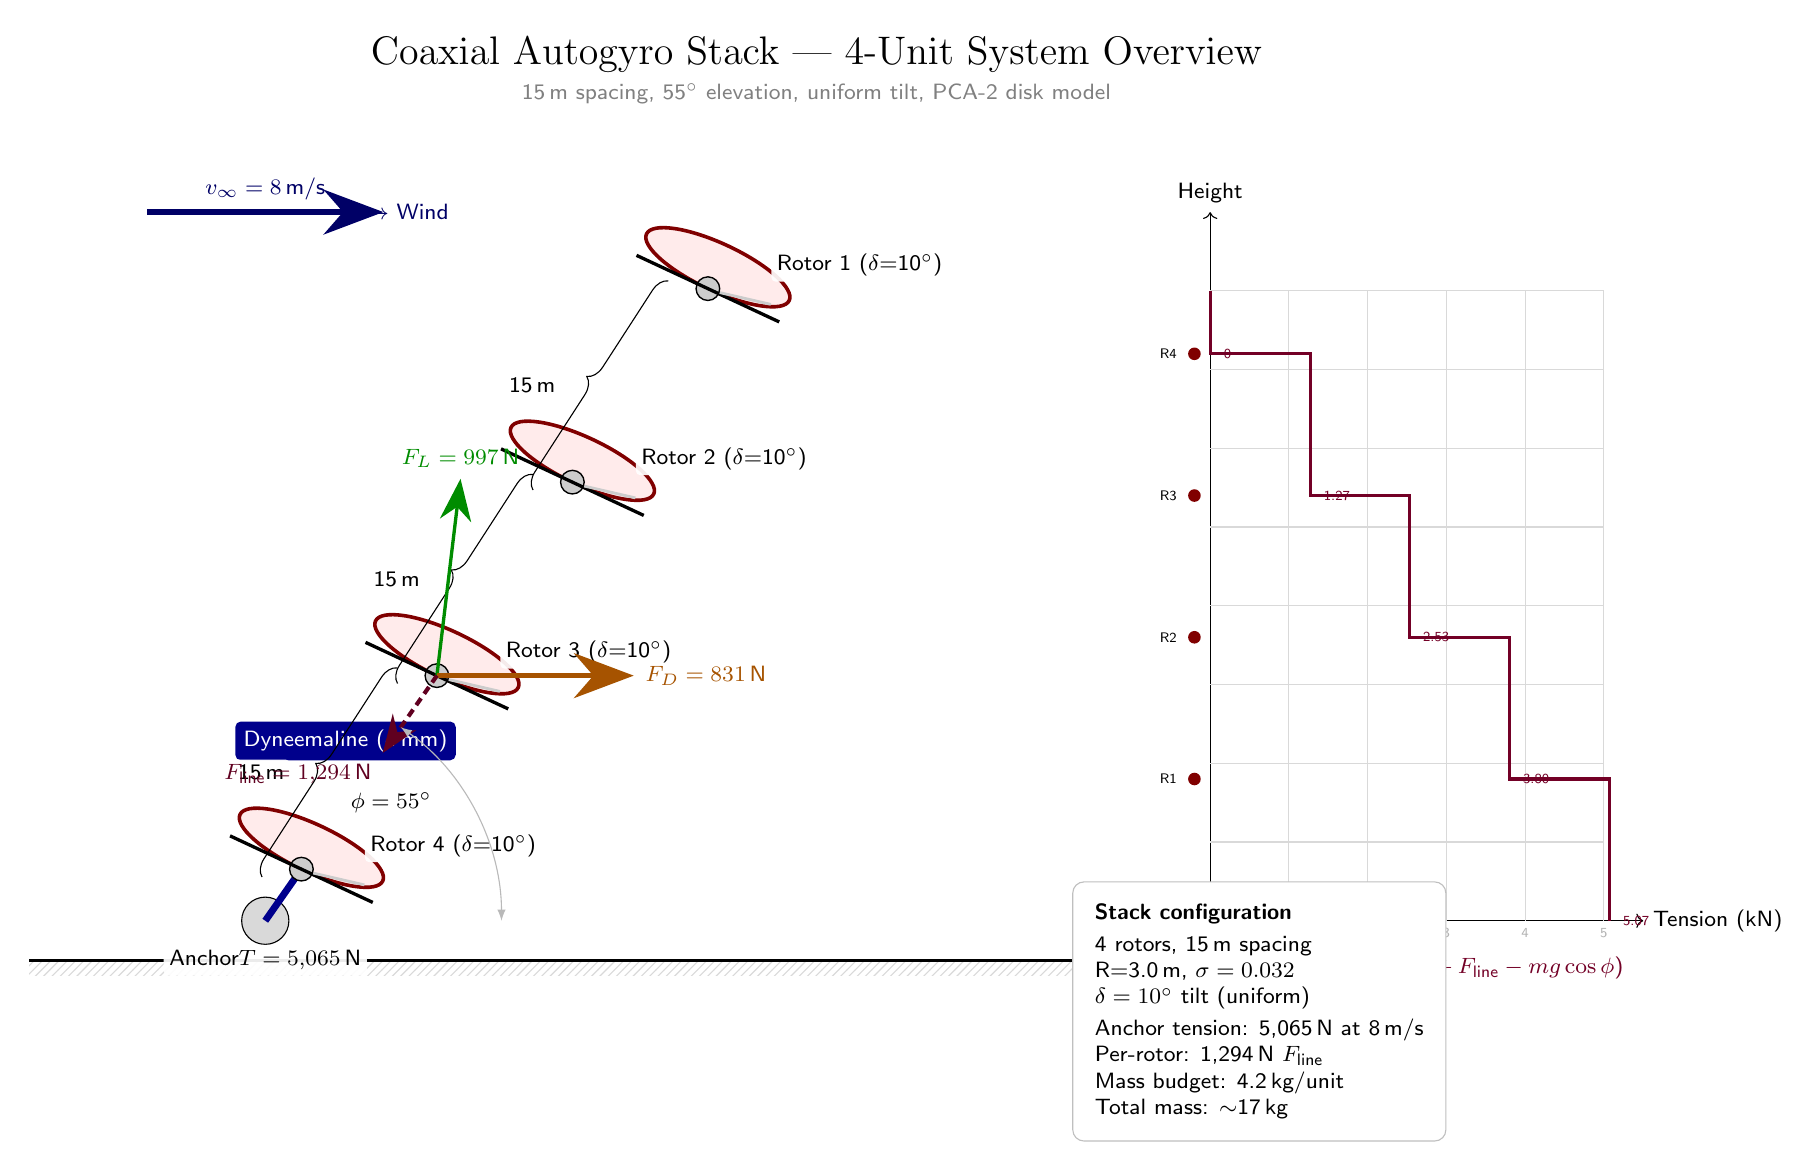
\begin{tikzpicture}[
    scale=1.0,
    dyneema/.style={draw=blue!55!black, line width=2.5pt},
    rotor/.style={draw=red!50!black, fill=red!8, line width=1.3pt},
    blade/.style={draw=red!40!black, fill=red!5, line width=1.2pt},
    force/.style={-{Stealth[scale=1.8]}, line width=2.0pt},
    forcecomp/.style={-{Stealth[scale=1.4]}, line width=1.5pt, densely dashed},
    dimline/.style={latex-latex, thin, draw=gray!55},
    annot/.style={font=\footnotesize\sffamily, fill=white, fill opacity=0.92,
                  text opacity=1, inner sep=2pt, rounded corners=1.5pt},
    label/.style={font=\small\sffamily\bfseries},
]

% Geometry
\def\elev{55}          % line elevation (deg)
\def\tilt{10}          % disk tilt (deg)
\def\spacing{3.0}      % visual spacing between rotors (cm)
\def\rotorR{1.0}       % visual rotor radius (cm)
\def\anchorX{1.0}      % anchor X position
\def\anchorY{0.5}      % anchor Y position

% Line direction vector
\pgfmathsetmacro{\dx}{cos(\elev)}
\pgfmathsetmacro{\dy}{sin(\elev)}

% Rotor positions along the line
% Bottom rotor (index 3, closest to anchor) through top rotor (index 0)
\foreach \i in {0,1,2,3} {
    \pgfmathsetmacro{\rx}{\anchorX + (0.8 + \i*\spacing)*\dx}
    \pgfmathsetmacro{\ry}{\anchorY + (0.8 + \i*\spacing)*\dy}
    \coordinate (R\i) at (\rx, \ry);
}

% ============================================================
% GROUND + ANCHOR
% ============================================================
\fill[pattern=north east lines, pattern color=black!15] (-2.0,-0.2) rectangle (16.0,0);
\draw[line width=1pt] (-2.0,0) -- (16.0,0);
\filldraw[fill=gray!30, draw=black] (\anchorX, \anchorY) circle (0.3);
\node[annot, below=0.3cm] at (\anchorX, \anchorY) {Anchor\\$T=5,\!065$\,N};

% ============================================================
% DYNEMA LINE --- terminates at top rotor R0
% ============================================================
\draw[dyneema] (\anchorX, \anchorY) -- (R0);
\node[font=\footnotesize\sffamily, fill=blue!55!black, text=white, inner sep=3pt, rounded corners=2pt] at ($(R0)!0.5!(R1) + (-0.3, 0.4)$) {Dyneema\\line (4\,mm)};

% ============================================================
% WIND ARROW --- horizontal, rightward
% ============================================================
\draw[force, blue!40!black, line width=2.0pt]
    (-0.5, 9.5) -- (2.5, 9.5)
    node[midway, above, font=\footnotesize\sffamily, blue!40!black] {$v_\infty=8$\,m/s};
\node[font=\footnotesize\sffamily, blue!40!black] at (2.8, 9.5) {$\to$ Wind};

% ============================================================
% ROTORS --- top to bottom (R0 = topmost, terminates line)
% ============================================================
\foreach \i in {0,1,2,3} {
    % Disk tilt: windward edge UP (CW rotation around center)
    \pgfmathsetmacro{\diskangle}{\elev + 90 + \tilt}  % tilt: windward edge UP
    \begin{scope}[shift={(R\i)}]
        % Rotor disk (ellipse)
        \fill[rotor, rotate=\diskangle]
            (0, -\rotorR*0.3) ellipse ({\rotorR} and {\rotorR*0.3});
        % Hub
        \filldraw[fill=gray!40, draw=black, line width=0.5pt] (0,0) circle (0.15);
        % Blade line
        \draw[line width=1.2pt, rotate=\diskangle]
            (-\rotorR, 0) -- (\rotorR, 0);
        % Empennage stub (downwind)
        \draw[gray!40, line width=1.0pt] (0.15, -0.05) -- (0.8, -0.2);
    \end{scope}

    % Label
    \pgfmathsetmacro{\inum}{int(4-\i)}
    \node[annot, right=0.3cm] at ($(R\i) + (0.5, 0.3)$)
        {Rotor \inum\ ($\delta$=\tilt$^\circ$)};

    % Spacing dimension
    \ifnum\i<3
        \pgfmathsetmacro{\nx}{int(\i+1)}
        \draw[decorate, decoration={brace, amplitude=6pt}]
            ($(R\i) + (-0.5, -0.1)$) -- ($(R\nx) + (-0.5, 0.1)$)
            node[midway, left=0.5cm, annot] {15\,m};
    \fi
}

% ============================================================
% FORCE ARROWS on middle rotor (R1)
% ============================================================
% F_lift --- green, upward from disk
\draw[force, green!55!black, very thick]
    (R1) -- ++(0.3, 2.5)
    node[above, font=\footnotesize\sffamily, green!55!black] {$F_L=997$\,N};

% F_drag --- orange, horizontal
\draw[force, orange!65!black]
    (R1) -- ++(2.5, 0)
    node[right, font=\footnotesize\sffamily, orange!65!black] {$F_D=831$\,N};

% F_line --- purple, along line toward anchor
\draw[forcecomp, purple!50!black]
    (R1) -- ++({-1.2*\dx}, {-1.2*\dy})
    node[below left, font=\footnotesize\sffamily, purple!50!black] {$F_\text{line}=1,\!294$\,N};

% ============================================================
% TENSION PROFILE --- staircase on the right
% ============================================================
\begin{scope}[shift={(13.0, 0.5)}]
    % Axes
    \draw[->] (0,0) -- (0,9.0) node[above, font=\footnotesize\sffamily] {Height};
    \draw[->] (0,0) -- (5.5,0) node[right, font=\footnotesize\sffamily] {Tension (kN)};

    % Grid
    \foreach \y in {1,2,3,4,5,6,7,8} {
        \draw[gray!30] (0,\y) -- (5.0,\y);
    }
    \foreach \x in {1,2,3,4,5} {
        \draw[gray!30] (\x,0) -- (\x,8.0);
        \node[font=\tiny\sffamily, gray!60] at (\x, -0.15) {\x};
    }

    % Tension staircase (increases downward)
    % Profile values from Julia model: 0, 1.27, 2.53, 3.80, 5.07 kN
    \draw[purple!60!black, very thick]
        (0, 8.0) -- (0, 7.2)               % top rotor $\rightarrow$ 0
        -- (1.27, 7.2) -- (1.27, 5.4)      % rotor 1 $\rightarrow$ 1.27 kN
        -- (2.53, 5.4) -- (2.53, 3.6)      % rotor 2 $\rightarrow$ 2.53 kN
        -- (3.80, 3.6) -- (3.80, 1.8)      % rotor 3 $\rightarrow$ 3.80 kN
        -- (5.07, 1.8) -- (5.07, 0.0);     % anchor $\rightarrow$ 5.07 kN

    % Annotations
    \node[font=\tiny\sffamily, purple!60!black, right=0.05cm] at (0, 7.2) {0};
    \node[font=\tiny\sffamily, purple!60!black, right=0.05cm] at (1.27, 5.4) {1.27};
    \node[font=\tiny\sffamily, purple!60!black, right=0.05cm] at (2.53, 3.6) {2.53};
    \node[font=\tiny\sffamily, purple!60!black, right=0.05cm] at (3.80, 1.8) {3.80};
    \node[font=\tiny\sffamily, purple!60!black, right=0.05cm] at (5.07, 0.0) {5.07};

    % Labels
    \node[font=\footnotesize\sffamily, purple!60!black] at (2.5, -0.6)
        {Tension ($T_\text{below}=T_\text{above}+F_\text{line}-mg\cos\phi$)};

    % Rotor markers
    \foreach \y/\lab in {7.2/4, 5.4/3, 3.6/2, 1.8/1} {
        \fill[red!50!black] (-0.2, \y) circle (0.08);
        \node[font=\tiny\sffamily, left=0.1cm] at (-0.2, \y) {R\lab};
    }
\end{scope}

% ============================================================
% ELEVATION ANGLE ARC
% ============================================================
\coordinate (horiz) at ($(\anchorX, \anchorY) + (4.5, 0)$);
\draw[dimline] (\anchorX, \anchorY) ++(3.0, 0) arc[start angle=0, end angle=\elev, radius=3.0cm];
\node[annot] at ($(\anchorX, \anchorY) + (1.6, 1.5)$) {$\phi=55^\circ$};

% ============================================================
% INFO PANEL --- bottom right
% ============================================================
\node[draw=black!25, fill=white, rounded corners=4pt, inner sep=8pt,
      anchor=north east, font=\footnotesize\sffamily, align=left]
    at (16.0, 1.0) {
    \textbf{Stack configuration}\\[2pt]
    4 rotors, 15\,m spacing\\
    R=3.0\,m, $\sigma=0.032$\\
    $\delta=10^\circ$ tilt (uniform)\\[2pt]
    Anchor tension: 5,065\,N at 8\,m/s\\
    Per-rotor: 1,294\,N $F_\text{line}$\\
    Mass budget: 4.2\,kg/unit\\
    Total mass: $\sim$17\,kg
};

% ============================================================
% TITLE
% ============================================================
\node[label, font=\Large] at (8.0, 11.5)
    {Coaxial Autogyro Stack --- 4-Unit System Overview};

\node[font=\footnotesize\sffamily, gray] at (8.0, 11.0)
    {15\,m spacing, 55$^\circ$ elevation, uniform tilt, PCA-2 disk model};

\end{tikzpicture}
\end{document}
